% =====================================================================
\chapter{A modellek kiértékelése}
\label{ch:modellek}
% =====================================================================

Az előző fejezet a módszer lépéseinek hatását vizsgálta modellenként; ez a fejezet a modelleket veti össze
egymással. Az olvasó megtudja belőle, (1) hogyan teljesít a három helyi modell \emph{azonos dokumentumokon},
(2) mennyire közelíti meg egy helyi modell a nagy szervermodellt, (3) miért bukott el a magyarra
továbbelőtanított PULI-LlumiX, és (4) mekkora kártya kell az egyes modellekhez, és milyen relatív költséggel
futnak. Mivel a három vizsgálat más dokumentumokon futott, modellek között csak azonos dokumentumhalmazon
hasonlítunk, és mindenhol megnevezzük, melyiken.

% =====================================================================
\section{A három helyi modell azonos dokumentumokon}
\label{sec:modellek-kozos}
% =====================================================================

\begin{sloppypar}
Két dokumentumhalmazon futott több modell is. (a) Az előzetes vizsgálat hat dokumentumán
(\code{en-economics-short-01}, \code{en-humanities-medium-02}, \code{en-law-long-03}, \code{hu-coffee},
\code{hu-gametheory}, \code{hu-immune}) a Qwen2.5-7B és a szervermodell futott, és mivel ez a hat
dokumentum a fő vizsgálat 30 dokumentuma között is szerepel, a PULI-LlumiX és a Gemma eredménye ezekre
leszűkítve is számolható. (b) A fő vizsgálat 30 dokumentumán a PULI-LlumiX és a Gemma futott.
\Az{\ref{tab:modellek-kozos}}.~táblázat az (a) halmazt mutatja.
\end{sloppypar}

\begin{table}[htbp]
\centering
\caption[A modellek minőségi indexe a hat közös dokumentumon.]{A modellek minőségi indexe ($Q$) a hat közös
dokumentumon (az előzetes vizsgálat dokumentumai; a PULI-LlumiX 8B és a Gemma 3 12B értéke a fő vizsgálat
futásaiból, erre a hat dokumentumra leszűkítve). $p$: páros Wilcoxon-próba a hat dokumentumon, korrigálatlan,
leíró jellegű (hat dokumentumon a legkisebb elérhető érték $0{,}031$). Szerver: a szervermodell ugyanazzal a
konfigurációval (\arm{B-doc-S}, \arm{E4}, \arm{E4b}).
$^a$Csak a három közös angol dokumentumon.}
\label{tab:modellek-kozos}
\small
\setlength{\tabcolsep}{4pt}
\begin{tabular}{@{}lcccccl@{}}
\toprule
Konfig. & \makecell{Qwen2.5\\7B} & \makecell{PULI-\\LlumiX 8B} & \makecell{Gemma 3\\12B} & \makecell{$p$ (Qwen--\\PULI)} & \makecell{$p$ (Qwen--\\Gemma)} & Szerver \\
\midrule
\arm{B-doc-L} & 0,83 & 0,49 & 0,97 & 0,031 & 0,031 & 0,95 (\arm{B-doc-S}) \\
\arm{E0}      & 0,64 & 0,32 & 0,71 & 0,031 & 0,094 & 0,94$^a$ (\arm{E4}) \\
\midrule
\arm{E1}      & 0,88 & 0,59 & 0,95 & 0,031 & 0,22  & -- \\
\arm{E2}      & 0,96 & 0,72 & 0,97 & 0,063 & 0,66  & 1,00$^a$ (\arm{E4b}) \\
\arm{E3}      & 0,88 & 0,44 & 0,97 & 0,031 & 0,22  & -- \\
\midrule
\arm{E2f}     & 0,90 & 0,69 & 0,98 & 0,031 & 0,094 & -- \\
\arm{E2h}     & 0,92 & 0,63 & 0,96 & 0,063 & 0,094 & -- \\
\arm{E2x}     & 0,89 & 0,71 & 0,96 & --    & --    & -- \\
\midrule
\arm{E5a}     & 0,87 & 0,36 & 0,97 & 0,031 & 0,031 & -- \\
\arm{E5b}     & 0,70 & 0,23 & 0,76 & 0,031 & 0,31  & -- \\
\arm{E5c}     & 0,86 & 0,29 & 0,97 & 0,031 & 0,69  & -- \\
\bottomrule
\end{tabular}
\end{table}

\paragraph{A hat közös dokumentumon} a sorrend minden konfigurációban azonos: Gemma $>$ Qwen $>$ PULI. A Qwen
a PULI-nál minden összevetett konfigurációban jobb, nyolcban mind a hat dokumentumon ($p=0{,}031$, a hat
dokumentumon elérhető legkisebb érték), az \arm{E2}-ben és az \arm{E2h}-ban $p=0{,}063$ mellett. A Gemma a
Qwennél minden konfigurációban magasabb értéket ért el, de egyöntetűen csak a teljes dokumentumos promptnál és az
\arm{E5a}-nál; a különbség az \arm{E2}-nél a legkisebb ($0{,}96$ vs.\ $0{,}97$, $p=0{,}66$), a teljes
dokumentumos promptnál a legnagyobb ($0{,}83$ vs.\ $0{,}97$). A három saját magyar szövegen is ez a kép:
az \arm{E2}-vel a Qwen $0{,}96$-ot, a PULI $0{,}74$-et, a Gemma $0{,}97$-et ért el, a naiv RAG-gal $0{,}88$-at,
$0{,}39$-et és $0{,}99$-et. A magyar nyelvre specializált modell tehát a magyar szövegeken is a leggyengébb volt.

\paragraph{A fő vizsgálat 30 dokumentumán} a Gemma a PULI-nál mind a tíz összevetett konfigurációban jobb (páros
Wilcoxon, korrigálatlanul $p\le5{,}3\cdot10^{-6}$; az értékeket \az{\ref{tab:fo}}.~táblázat adja). A különbség a
tervezett és ellenőrzött folyamatnál a legkisebb (\arm{E2}: $0{,}67$ vs.\ $0{,}95$), és az egyhívásos
konfigurációkban a legnagyobb (\arm{E5c}: $0{,}25$ vs.\ $0{,}97$): a módszer a két modell közötti távolságot
csökkenti, de nem tünteti el.

% =====================================================================
\section{A szervermodell és a helyi modellek}
\label{sec:modellek-szerver}
% =====================================================================

A szervermodell (az egyetemi GenAI-szerver nagy Qwen-modellje) csak az előzetes vizsgálatban futott. A teljes
dokumentumos prompttal (\arm{B-doc-S}, a mai gyakorlat) a hat közös dokumentumon $0{,}95$-öt ért el
(95\,\%-os intervallum $0{,}87$--$0{,}99$), a naiv RAG-gal (\arm{E4}) a saját hat angol dokumentumán $0{,}91$-et
($0{,}80$--$0{,}98$), a mi tervezett és ellenőrzött folyamatunkkal (\arm{E4b}) $0{,}99$-et ($0{,}97$--$1{,}00$); a
három közös angol dokumentumon $0{,}94$-et, illetve $1{,}00$-t.

A helyi Qwen2.5-7B a tervezett és ellenőrzött folyamattal (\arm{E2}, $0{,}96$) a hat közös dokumentumon tehát
eléri a szervermodell teljes dokumentumos promptját ($0{,}95$), a három közös angol dokumentumon pedig a
szervermodell naiv RAG-ját ($0{,}95$ vs.\ $0{,}94$). Ugyanezzel a módszerrel azonban a szervermodell is jobb lesz
($0{,}99$): a „helyi modell eléri a szervermodellt” állítás csak a szervermodell teljes dokumentumos
promptjára igaz, a módszert alkalmazó szervermodellre nem. A különbségek hat, illetve három dokumentumon
születtek, ezért leírók; szignifikanciát ezen a mintán Holm-korrekció után elvileg sem lehet kimutatni
(\ref{sec:statisztika}.~szakasz).

A szervermodell a módszerrel minden más mutatón is a legjobb volt: kérdéshelyeinek 83\,\%-a elsőre átment az
ellenőrzésen (a Qwennél 23\,\%), a bíró a kérdések 98\,\%-ára mondta, hogy felhasználná (Qwen \arm{E2}: 80\,\%),
és a tervezett és megvalósult Bloom-szint 62\,\%-ban egyezett (Qwen: 35\,\%). Naiv RAG-gal viszont a szervermodell
is a naiv RAG hibáit mutatta: a kérdéspárok 49\,\%-a közel azonos volt, a lefedettség 9\,\% (\arm{E4b}: 28\,\%),
és formailag hibátlan, de tartalmilag üres kérdéseket is írt („Hány szóból áll a »Link to Learning« cím?”),
amelyeket a bíró 5/5-re pontozott. Ez ugyanaz a szerkezeti darab, amely a helyi naiv RAG-ot is félrevitte
(\ref{sec:fo-robusztus}.~szakasz), és a szivárgáshoz hasonlóan a mérést felfelé torzítja. Futásidőt a megosztott
szerveren mért értékekből nem hasonlítunk a helyiekhez; a szerver saját \arm{E4b}/\arm{E4} szorzója kb.\ 9.

% =====================================================================
\section{Miért bukik el a PULI-LlumiX?}
\label{sec:fo-puli}
% =====================================================================

A magyarra továbbelőtanított modelltől azt vártuk, hogy a magyar dokumentumokon jobb lesz a többnyelvű
modelleknél. Ehelyett a vizsgálat leggyengébb modellje lett, a magyar szövegeken is
(\ref{sec:modellek-kozos}.~szakasz), és ennek oka nem a nyelv, hanem az \emph{utasításkövetés}.

\paragraph{A modell.} A modellkártya szerint a PULI-LlumiX-Llama-3.1 a Llama 3.1 8B \emph{Instruct} modell
magyar szövegeken folytatott továbbelőtanítása, utólagos utasítás-hangolás nélkül; a kártya „base” modellnek
nevezi~\cite{pulillumix}. A vizsgálatban nem a fejlesztő által közzétett súlyok, hanem egy harmadik féltől
származó, GGUF formátumú, kvantált változat futott ({\small\nolinkurl{hf.co/mradermacher/PULI-LlumiX-Llama-3.1-GGUF:Q4_K_M}},
\ref{app-reprodukcio}.~függelék).

\paragraph{A tünetek.} Egyetlen hívásban a PULI a kért tíz kérdés helyett átlagosan 1,8-at (\arm{E0}), illetve
5,6-ot (\arm{B-doc-L}) adott vissza; az egyhívásos konfigurációk formai megfelelése 1--6\,\%, vagyis a vizsgák
94--99\,\%-a formailag hibás volt, a darabolási változatok vizsgáinak 14--29\,\%-ában pedig a válasz nem is volt
értelmezhető JSON. A tervezett folyamat ezt részben megkerüli, mert egy hívásban csak egy kérdést kér, de a
tervezett konfigurációk futása során is konfigurációnként 128--620 modellválasz nem volt értelmezhető (a
Gemmánál és a Qwennél egy sem). A kérdések minősége így is gyenge marad: az ellenőrzés nélküli \arm{E1}
kérdéseinek 34\,\%-a szivárogtatja a kulcsot, 45\,\%-ának törzse nem kérdés, a kérdéspárok 62\,\%-a közel azonos,
a törzsek pedig átlagosan 252 karakteresek (a Gemma \arm{E1}-ében 122). A modell jellemzően a forrás egy mondatát
másolja be kérdésként és kulcsként is -- ugyanazt a hibát mutatva, amelyet a pilot a Qwen-ellenőrző
visszacsatolásánál talált (\ref{sec:szivargas}.~szakasz). A \emph{Nürnbergi per} cikkből például a „kérdés” a
forrás egy kijelentő mondata volt, és a négy válaszlehetőség közül kettő ugyanez a mondat; a bíró helyességi
pontszáma 1/5 lett.

Az ellenőrző lánc a szivárgást (34\,\%$\to$12\,\%) és a nem kérdő törzseket (45\,\%$\to$22\,\%) mérsékli, de
nem szünteti meg, a megvalósult Bloom-szint gyakorlatilag mindig az emlékezés marad, és a teljes módszerrel is 18
dokumentumon $0{,}70$ alatt marad a minőségi index (a leggyengébben $0{,}38$). Az \arm{E1} futása emellett
instabil volt: 103 modellhívás időtúllépéssel vagy hibával zárult, és egy vizsga medián ideje 96 perc lett (a
Gemmánál 2,9 perc).

\paragraph{Mire általánosítható?} A következtetés erre a modellre szűkül: nem általában a magyar nyelvű
továbbtanítás, hanem ez a továbbelőtanított, utána újra nem hangolt modell (ebben a kvantált változatban) nem
követte a strukturált kimenet formátumát. Feltevésként megemlíthető, hogy a csevegési sablon (chat-sablon) is
szerepet játszhatott, vagyis hogy a GGUF-fájlba ágyazott sablon eltért attól, amellyel a modell a legjobban
működik; ezt nem vizsgáltuk, és a kvantálás hatását sem tudjuk elkülöníteni. A gyakorlati tanulság: a
modellválasztásnál egy strukturált, formátumkövető feladathoz az utasításkövetés legalább olyan fontos, mint a
nyelvi teljesítmény, és ezt a célfeladaton kell mérni.

% =====================================================================
\section{Erőforrásigény és GPU-szintek}
\label{sec:fo-eroforras}
% =====================================================================

\Az{\ref{tab:eroforras}}.~táblázat a három helyi modell mért memóriaigényét és azonos kártyán mért relatív
futási idejét foglalja össze; \az{\ref{fig:minoseg-ido}}.~ábra a minőséget a futási idő függvényében mutatja.

\begin{table}[htbp]
\centering
\caption[A helyi modellek erőforrásigénye.]{A helyi modellek erőforrásigénye. Modell: az Ollama által
jelentett, mért foglalás 8\,192 tokenes kontextusnál (GiB; a \ref{tab:budget}.~táblázat becslésével
összevetendő); Teljes dok.: ugyanez a 16\,384 tokenes \arm{B-doc-L} konfigurációnál; Kártya: a szükséges
fogyasztói GPU az asztali környezet 1,6--1,9\,GiB-os foglalása mellett (a pilot mérése); \arm{E2}/\arm{E0}: a
medián vizsgaidő modellen belüli szorzója ugyanazon a kártyán (\ref{tab:koltseg}.~táblázat).}
\label{tab:eroforras}
\small
\begin{tabular}{@{}lcccc@{}}
\toprule
Modell & Modell (GiB) & Teljes dok.\ (GiB) & Kártya & \arm{E2}/\arm{E0} \\
\midrule
Qwen2.5-7B (Q4\_K\_M)     & 4,8 & 5,2 & 8\,GB-os           & 10,9$\times$ \\
PULI-LlumiX 8B (Q4\_K\_M) & 5,5 & 6,5 & 8\,GB-os$^\ast$    & 52,3$\times$ \\
Gemma 3 12B (Q4\_K\_M)    & 7,8 & 7,8 & 12\,GB-os          & 8,5$\times$ \\
\bottomrule
\end{tabular}

\smallskip
{\footnotesize $^\ast$ A 16\,384 tokenes teljes dokumentumos konfigurációhoz a 8\,GB-os kártya várhatóan nem
elég (lásd a szöveget).\par}
\end{table}

\paragraph{Memória.} A Qwen2.5-7B (4,8\,GiB) és a PULI-LlumiX 8B (5,5\,GiB) 8\,192 tokenes kontextussal egy
8\,GB-os fogyasztói kártyán is elfér (a pilot asztali gépén, RTX 3070 Ti mellett a Qwennel a legrosszabb esetben
is kb.\ 380\,MiB tartalék maradt); a Gemma 3 12B 7,8\,GiB-os foglalása az asztali környezettel együtt kb.\
9,4--9,7\,GiB, vagyis egy 12\,GB-os fogyasztói kártyát igényel. A 16\,384 tokenes teljes dokumentumos
konfigurációnál a Qwen foglalása 464\,MiB-tal nőtt, ami nagyságrendben egyezik a \eqref{eq:vram} becslés
448\,MiB-os KV-többletével; a PULI-é 1\,024\,MiB-tal 6,5\,GiB-ra, így az asztali környezettel együtt egy
8\,GB-os kártya kapacitását meghaladná (fogyasztói kártyán ezt nem mértük). A Gemma foglalása gyakorlatilag nem nőtt (16\,MiB); ezt feltehetően a modell csúszóablakos helyi
figyelemrétegei magyarázzák~\cite{gemma3}, de nem vizsgáltuk.

\paragraph{Futási idő.} A futásidőt relatív szorzóként, egy vizsgálaton belül értelmezzük
(\ref{sec:fo-koltseg}.~szakasz): az abszolút percek más kártyán mások lennének, a szorzók érdemben nem. A
tervezett és ellenőrzött folyamat a Gemmánál az \arm{E0} idejének 8,5-szerese, a Qwennél 10,9-szerese. A
PULI szorzója ($52{,}3\times$) félrevezetően nagy, mert az \arm{E0}-ja alig ír kérdést; a fő vizsgálaton belül,
ugyanazon a 30 dokumentumon és kártyán mérve a PULI \arm{E0}-ja a Gemmáénak kb.\ 0,4-szerese, az \arm{E2}-je
viszont kb.\ 2,4-szerese. A PULI tehát kisebb modell létére a tervezett folyamatban lassabb, mert szinte minden
kérdéshelyet újra kell próbálnia (2,0 kísérlet a Gemma 1,3-ával szemben, \ref{tab:ellenorzo}.~táblázat), és sok
válasza értelmezhetetlen. A Qwen és a fő vizsgálat modelljeinek idejét nem vetjük össze, mert más vizsgálatban,
más dokumentumokon mértük.

\begin{figure}[htbp]
\centering
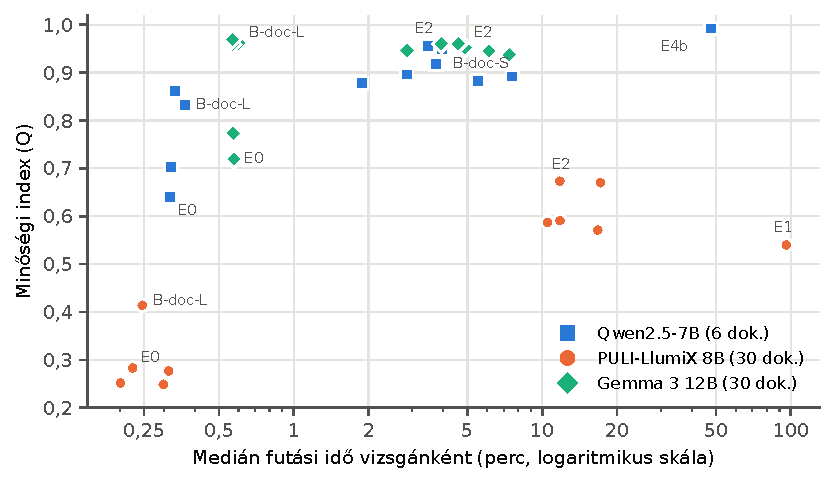
\includegraphics[width=0.9\textwidth]{figures/f4_minoseg_ido}
\caption[Minőség és futási idő.]{Minőség és futási idő. Az egyhívásos konfigurációk gyorsak, de minőségük a
modelltől és a darabolástól függően erősen ingadozik; a tervezett konfigurációk lassabbak, de minden modellnél a
legjobbak között vannak.}
\label{fig:minoseg-ido}
\end{figure}

\paragraph{GPU-szintek.} A mérések alapján két szint különíthető el: egy 8\,GB-os kártyán a 7--8B modellek
futnak, ezek közül a vizsgált feladatra a Qwen2.5-7B alkalmas; egy 12\,GB-os kártyán a Gemma 3 12B, amely minden
konfigurációban a legjobb helyi eredményt adta. Hogy melyik szinten melyik konfiguráció kerüljön a rendszerbe,
\az{\ref{ch:diszkusszio}}.~fejezet dönti el.

% =====================================================================
\section{Modellválasztási tanulság}
\label{sec:modellek-tanulsag}
% =====================================================================

Két tanulság emelhető ki. \emph{Először}, a vizsgált feladatban az utasításkövetés fontosabb volt a nyelvi
specializációnál: a többnyelvű Qwen2.5-7B a hat közös dokumentumon -- a magyar szövegeken is -- minden
konfigurációban jobb volt a magyarra továbbelőtanított PULI-LlumiX 8B-nél. \emph{Másodszor}, minél erősebb a
modell, annál kisebb a módszer haszna a minőségben: ugyanezen a hat dokumentumon a teljes módszer
(\arm{E2}--\arm{E0}) a PULI-nál $0{,}41$-dal, a Qwennél $0{,}32$-vel, a Gemmánál $0{,}26$-tal javított, a teljes
dokumentumos prompthoz képest (\arm{E2}--\arm{B-doc-L}) pedig $0{,}23$-dal, $0{,}12$-vel, illetve egyáltalán
nem. Az erős modellnél a módszer értéke ezért elsősorban az ellenőrizhetőség (kérdésenkénti forrás, terv,
ellenőrzés), a gyenge modellnél maga a használható vizsga. Mivel e tulajdonságokat a modellkártya nem mutatja meg,
a modellt a célfeladaton kell kiválasztani -- erre szolgál a dolgozat kiértékelő keretrendszere.
